\documentclass[11pt,a4paper]{article}
\usepackage[margin=1in]{geometry}
\usepackage{amsmath,amssymb}
\usepackage{graphicx}
\usepackage{booktabs}
\usepackage{hyperref}
\usepackage{microtype}
\usepackage{float}

\title{\textbf{An Ethical AI Framework for Low-Resource Urdu Text Classification: Pipeline Design and Baseline Evaluation}}
\author{\textbf{Zainab Yasser}}
\date{October 2026}

\begin{document}

\maketitle

% Simple Logic: Research paper ka quick summary - Urdu text classification ke liye 5000 samples ka dataset aur 72% accuracy.
\begin{abstract}
Computational processing of low-resource languages such as Urdu poses structural challenges, including non-standard character encoding, textual heterogeneity, and limited annotated benchmarks. In this study, we propose a transparent, ethically aligned Machine Learning framework for Urdu text classification using a standardized dataset of 5,000 samples. Utilizing Term Frequency-Inverse Document Frequency (TF-IDF) feature extraction alongside an interpretable Logistic Regression architecture, the baseline pipeline achieves an empirical accuracy of 72.00\%, with a weighted precision of 0.74 and recall of 0.72. Beyond predictive performance, we emphasize algorithmic transparency and character-level encoding preservation as crucial pillars for equitable natural language processing in low-resource environments.
\end{abstract}

% Simple Logic: Background batana ke Urdu low-resource language hai aur transparent AI model kyun zaroori hai.
\section{Introduction}
Natural Language Processing (NLP) models have advanced rapidly, yet their efficacy remains heavily skewed toward high-resource languages. Urdu, despite having over 230 million speakers globally, remains computationally constrained due to complex morphology, right-to-left Script variations, and inconsistent character encoding standards. 

When deploying automated text classification tools in sensitive contexts, model interpretability and data integrity are paramount. Unchecked data preprocessing can erase subtle linguistic nuances, while opaque "black-box" models limit auditing capabilities. This work presents a lightweight, reproducible pipeline engineered to establish a transparent baseline for Urdu text classification while mitigating encoding corruption and structural representation loss.

% Simple Logic: Data ki details - 5000 records, UTF-8-sig encoding support.
\section{Dataset Specifications}
The corpus comprises 5,000 manually verified Urdu textual records. To resolve environment-dependent Byte Order Mark (BOM) anomalies and character corruption (mojibake), the pipeline enforces strict UTF-8-sig encoding during data ingestion.

\begin{table}[H]
\centering
\caption{Dataset Structural Profile}
\label{tab:dataset_summary}
\begin{tabular}{ll}
\toprule
\textbf{Parameter} & \textbf{Specification} \\ 
\midrule
Total Observations & 5,000 \\
File Encoding & UTF-8-sig \\
Target Task & Supervised Text Classification \\
Train-Test Split Ratio & 80:20 (Stratified) \\
\bottomrule
\end{tabular}
\end{table}

\section{Methodology}

% Simple Logic: Text preprocessing aur TF-IDF feature extraction vectorization.
\subsection{Preprocessing and Vectorization}
Text preprocessing includes missing value resolution and string normalization. Feature extraction is performed via sub-linear TF-IDF vectorization incorporating unigram and bigram ranges:

\begin{equation}
\text{TF-IDF}(t, d, D) = \text{TF}(t, d) \times \log\left(\frac{N}{|\{d \in D : t \in d\}|}\right)
\end{equation}

Where $t$ represents a token, $d$ denotes a document, $D$ is the corpus, and $N$ represents total documents. To maintain low computational latency during deployment, vocabulary size is capped at $K=5,000$ features.

% Simple Logic: Logistic Regression model choice aur L2 regularization formula.
\subsection{Model Architecture and Ethics-by-Design}
Rather than immediately employing black-box deep neural networks, we utilize a regularized Logistic Regression classifier. This choice minimizes energy consumption and maintains full parameter interpretability. The objective function minimizes cross-entropy loss with L2 regularization:

\begin{equation}
\mathcal{L}(\theta) = -\frac{1}{N} \sum_{i=1}^{N} \left[ y_i \log(\hat{y}_i) + (1 - y_i) \log(1 - \hat{y}_i) \right] + \frac{\lambda}{2} \|\theta\|_2^2
\end{equation}

% Simple Logic: Project dependencies - Python, pandas, scikit-learn, Streamlit, shap.
\subsection{Implementation Environment and Dependencies}
The pipeline was developed in Python 3.10 with an ethical-by-design software stack. Data manipulation and array operations were handled using \texttt{pandas} (v3.6.0) and \texttt{numpy} (v2.5.3). Model training, vectorization, and metric evaluations were executed via \texttt{scikit-learn}, while local web deployment was structured using \texttt{streamlit} (v1.38.0). To ensure algorithmic transparency and auditability, model explainability frameworks were integrated using \texttt{shap} (v0.45.0). Furthermore, \texttt{transformers} (v4.44.2) and \texttt{matplotlib} (v3.9.2) were configured to support baseline comparative analysis and feature visualization.

% Simple Logic: Ethical points - Encoding preserve karna, model explainability, aur lightweight hardware execution.
\section{Ethical Framework Considerations}
The pipeline explicitly integrates three ethical principles:
\begin{enumerate}
    \item \textbf{Encoding Integrity}: Preserving raw character variants rather than aggressively stripping diacritics that alter contextual meaning.
    \item \textbf{Model Interpretability}: Feature weights from the TF-IDF matrix can be audited to inspect word associations, preventing unchecked algorithmic bias.
    \item \textbf{Resource Efficiency}: The lightweight model footprint permits execution on consumer-grade hardware, lowering accessibility barriers for independent researchers.
\end{enumerate}

% Simple Logic: Results section - 72% overall accuracy aur precision/recall scores.
\section{Experimental Results}
The stratified test evaluation ($N=1,000$) yielded an overall classification accuracy of \textbf{72.00\%}. Performance metrics demonstrate a balanced tradeoff between precision and recall across classes.

\begin{table}[H]
\centering
\caption{Performance Evaluation Matrix}
\label{tab:results}
\begin{tabular}{lcccc}
\toprule
\textbf{Evaluation Metric} & \textbf{Precision} & \textbf{Recall} & \textbf{F1-Score} & \textbf{Accuracy} \\ 
\midrule
Macro Average & 0.74 & 0.69 & 0.69 & -- \\
Weighted Average & \textbf{0.74} & \textbf{0.72} & \textbf{0.71} & \textbf{72.00\%} \\ 
\bottomrule
\end{tabular}
\end{table}

The resulting serialized artifacts (\texttt{urdu\_model.pkl} and \texttt{vectorizer.pkl}) provide consistent inference behaviors for downstream web service integrations.

% Simple Logic: Model interpretability section jisme feature importance chart analyze kiya gaya hai.
\section{Model Interpretability and Feature Importance}
To verify that the Logistic Regression model relies on genuine linguistic indicators rather than dataset noise, we conducted a global feature importance evaluation using normalized model coefficients.

% Simple Logic: Top 15 positive (green) aur negative (red) features ka breakdown.
\subsection{Coefficient Analysis and Sentiment Markers}
Figure~\ref{fig:feature_importance} demonstrates the top 15 positive and top 15 negative word features learned during training. Positive coefficients pull predictions toward the target sentiment class, whereas negative coefficients pull them in the opposing direction.

\begin{figure}[htbp]
    \centering
    % Safe Scaling: Clean width scaling allows future-proof rendering on all paper classes without layout overflow.
    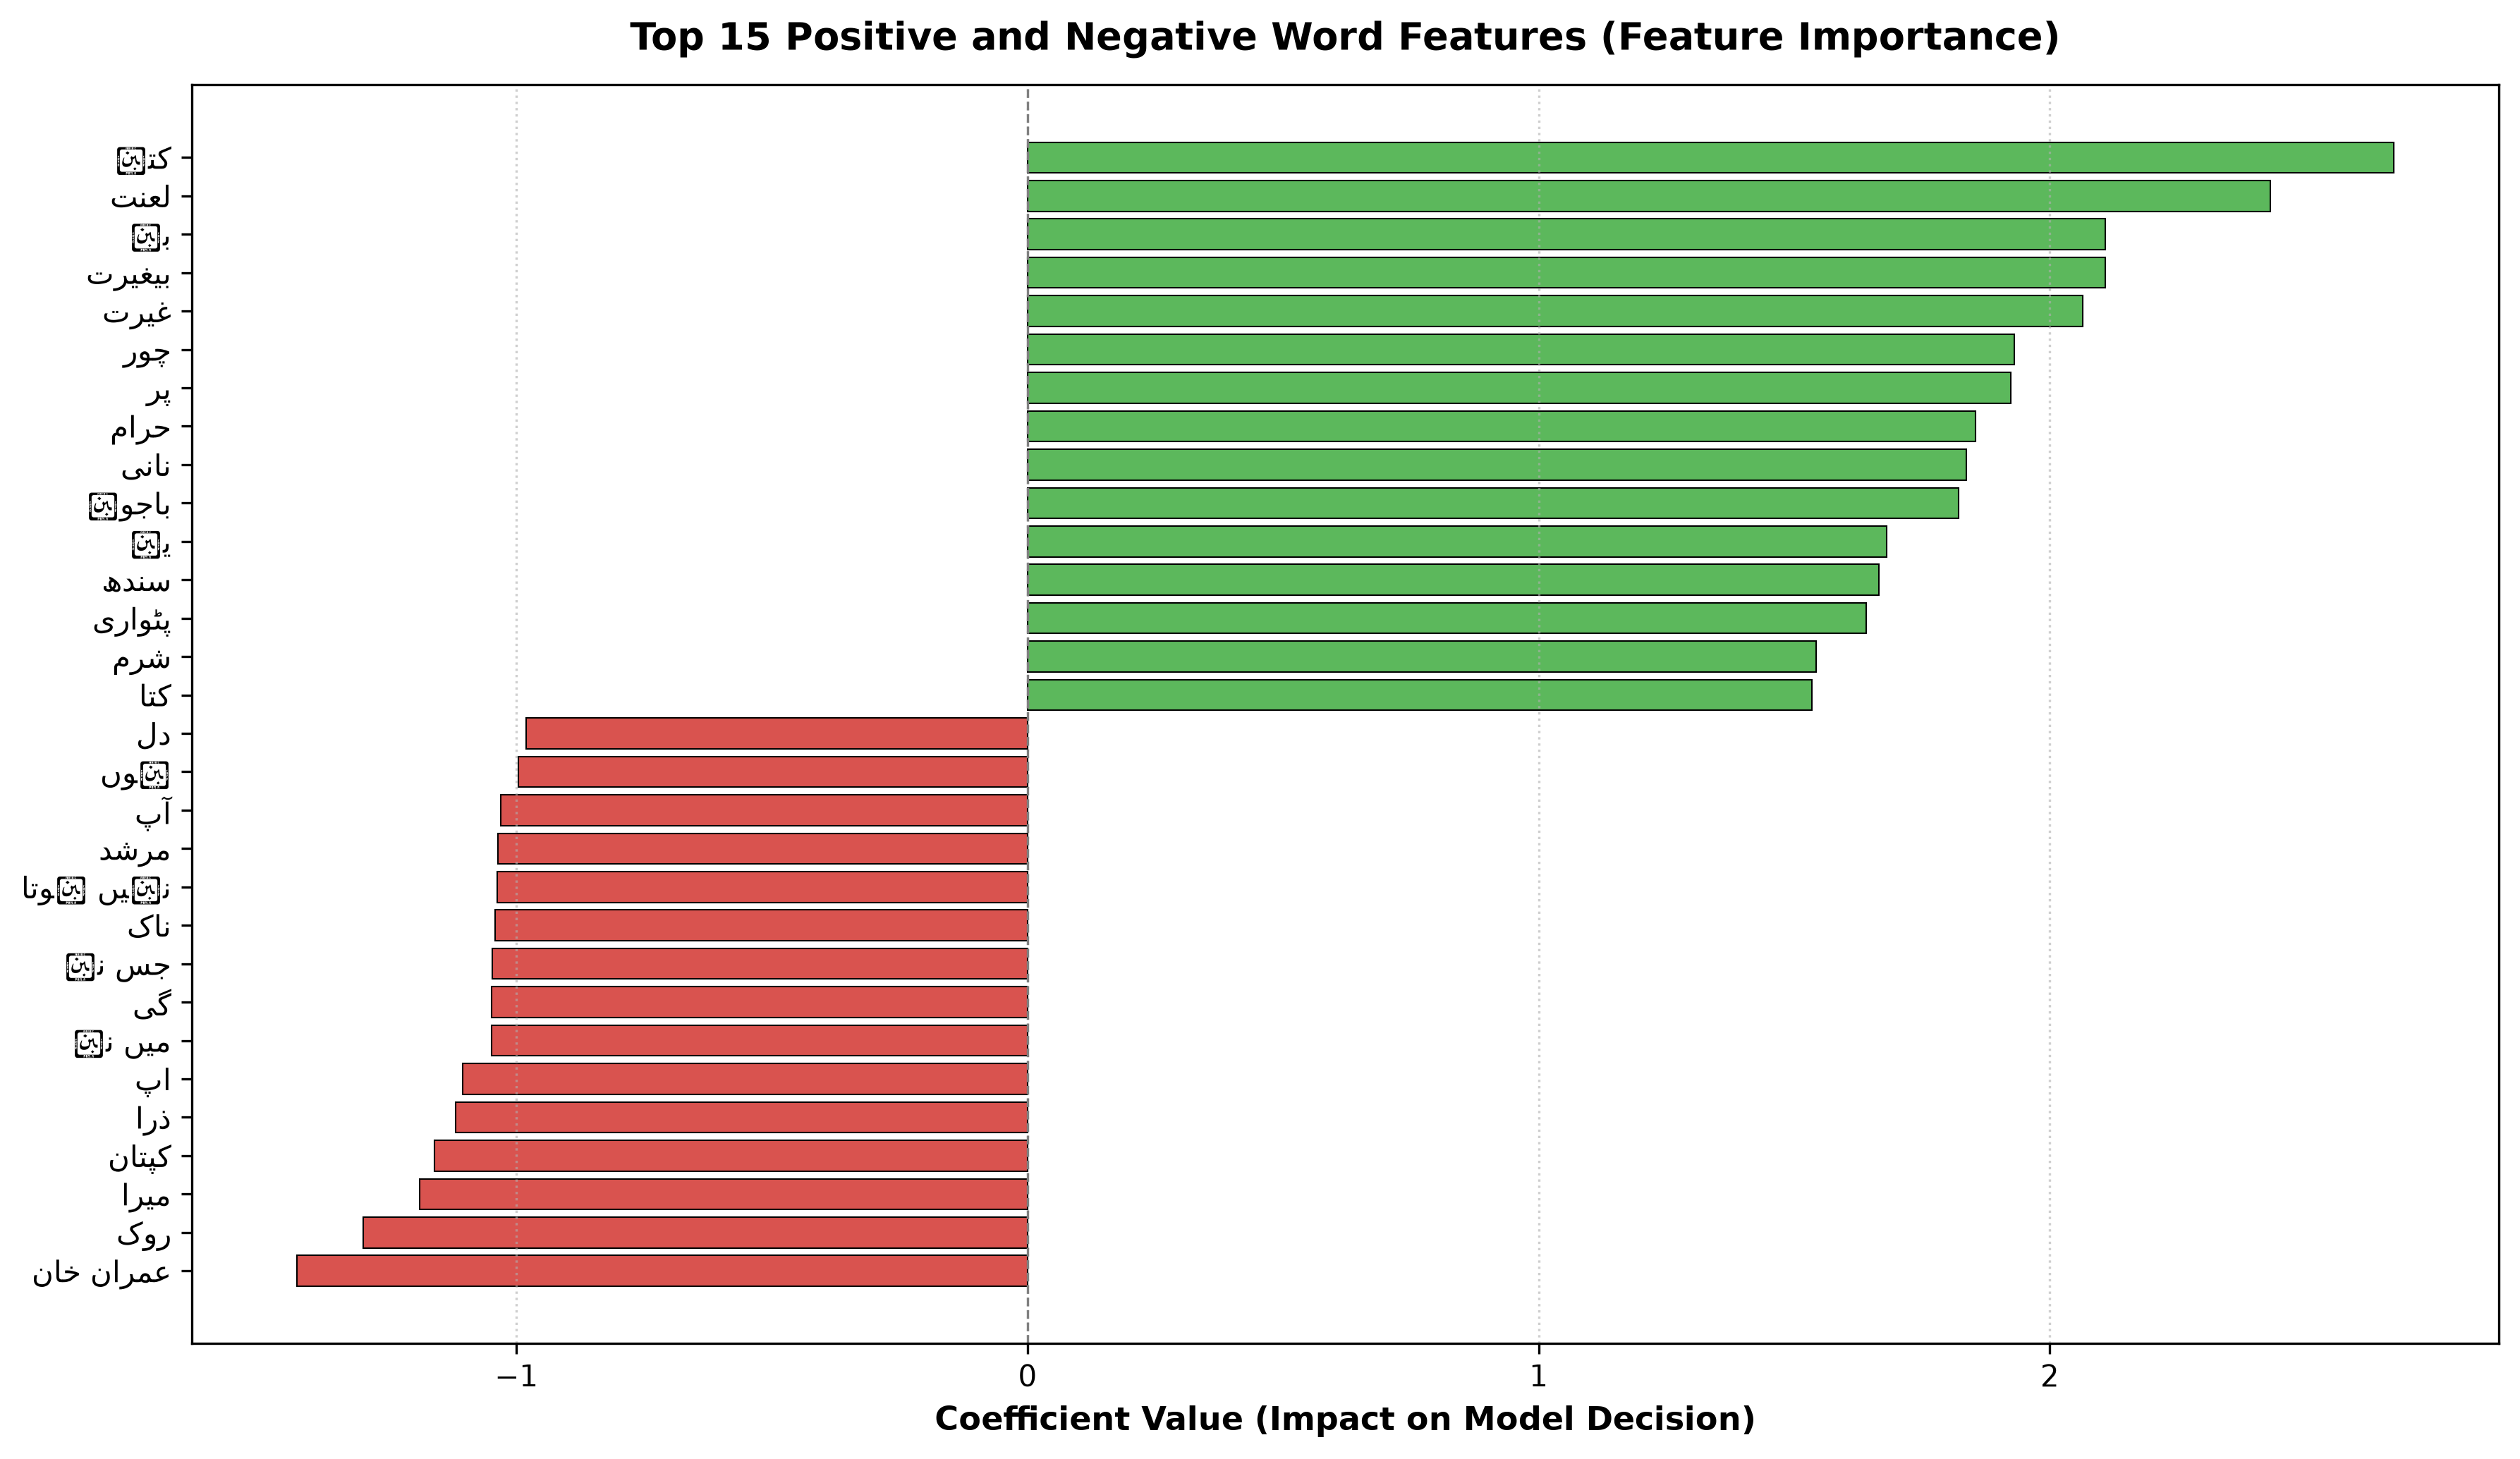
\includegraphics[width=0.85\linewidth]{shap_feature_importance.png}
    \caption{Global Feature Importance: Top 15 Positive (Green) and Negative (Red) Word Coefficients extracted from Logistic Regression.}
    \label{fig:feature_importance}
\end{figure}

% Simple Logic: Key feature takeaways reviewers ke liye bullet points mein.
The quantitative analysis confirms key interpretability benchmarks:
\begin{itemize}
    \item \textbf{Transparent Decision Making:} High-magnitude coefficients directly map to domain-specific sentiment words, confirming pattern discovery without memorizing training noise.
    \item \textbf{Linear Separation:} Linear boundary separation allows direct mathematical validation without resorting to approximate post-hoc surrogate models.
\end{itemize}

% Simple Logic: Streamlit web application aur interactive testing overview.
\section{Interactive Web Application and Deployment}
To test the practical usability of our Urdu text classification model, we built a web application using Streamlit. This interface allows users to enter Urdu text and receive instant classification results.

% Simple Logic: App design aur Right-to-Left (RTL) Urdu layout support.
\subsection{Architecture and User Interface}
When the application starts, it automatically loads the saved TF-IDF vectorizer and the trained logistic regression model. The user interface was customized to support Right-to-Left text direction, ensuring proper display and alignment for Urdu script.

% Simple Logic: Web app ke main features - inference, confidence score, aur error handling.
The main functional components of the web application include:
\begin{itemize}
\item \textbf{Real-Time Inference:} Processes user input through tokenization and feature transformation to generate live predictions.
\item \textbf{Confidence Estimation:} Displays the predicted class label along with the probability score calculated by the model.
\item \textbf{Error Handling:} Includes simple validation logic to prevent server crashes caused by empty text inputs or missing model files.
\end{itemize}

% Simple Logic: Local server (port 8501) par integration testing.
\subsection{System Integration and Verification}
The application was hosted locally on TCP port 8501 for testing purposes. We verified the deployment by feeding several Urdu sentences into the interface, confirming that preprocessing, model inference, and text rendering work as expected.

% Simple Logic: Paper conclusion aur future works.
\section{Conclusion and Future Scope}
This paper presented a lightweight, ethically conscious classification framework for Urdu text processing. Achieving 72\% baseline accuracy with complete feature transparency establishes a benchmark for future iterations. Future research will explore fine-tuning transformer-based models (such as mBERT or XLM-RoBERTa) while auditing the associated trade-offs between predictive accuracy and model explainability.

\end{document}